\documentclass[11pt]{beamer}
\usepackage{settings}

% Reduce inter-line spacing globally (affects most text)
\usepackage{setspace}
\renewcommand{\baselinestretch}{0.97}

\title[NEAT]{\vspace {2em}Pacman-NEAT: \\ Exploring the Power of Evolutionary Algorithms in Game Playing}
\subtitle{A Case Study with NEAT and Pacman}
\date{08/07/2025}
\author{Andrea Spinelli}
\institute{\vspace{-5em} University of Trieste \hfill 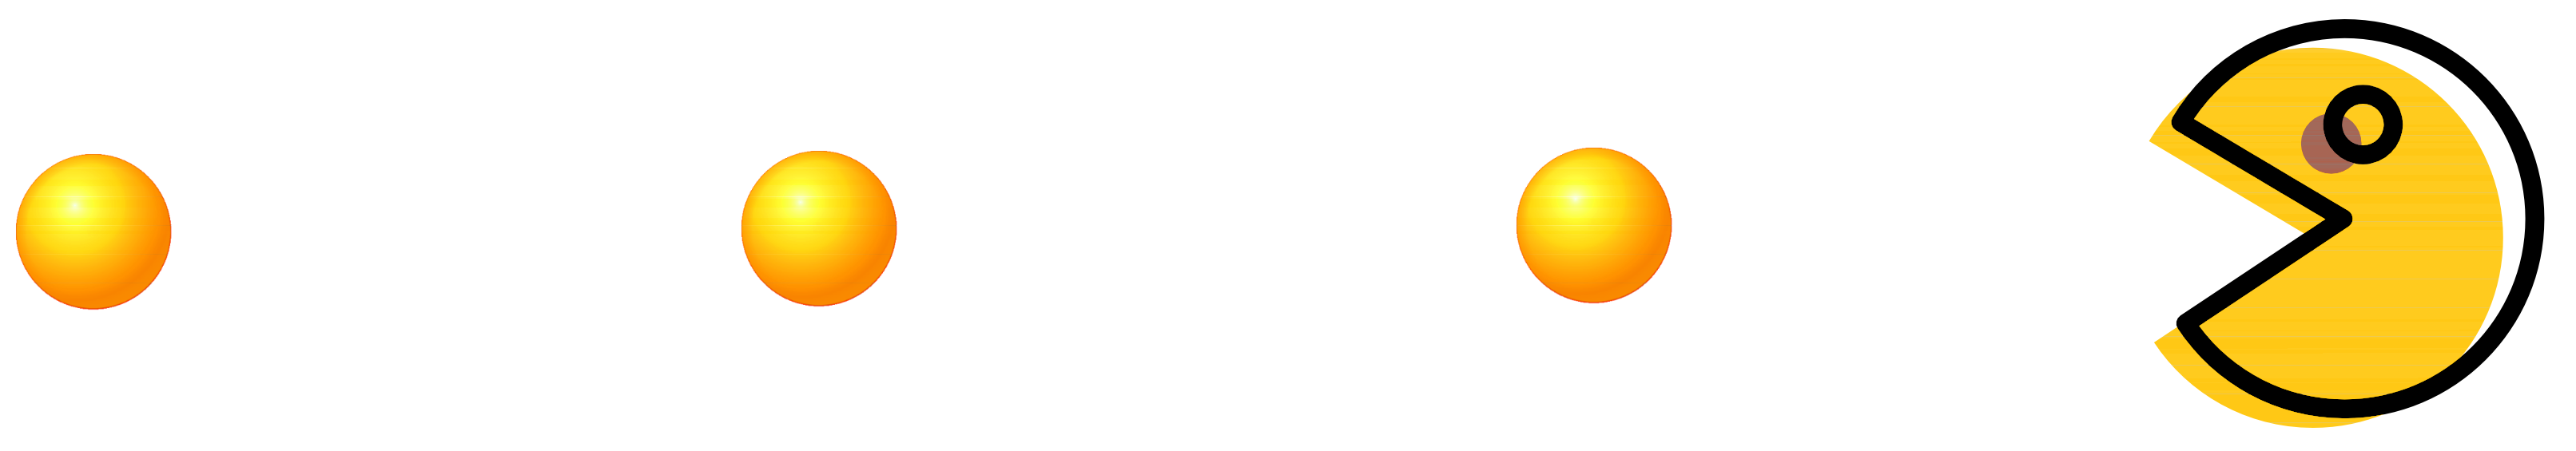
\includegraphics[height=1.5cm]{assets/pacman.png}}
\titlegraphic{\hfill
\includegraphics[height=1.5cm]{assets/logo100_orizzontale.pdf}}

\usepackage{xcolor}
\newcommand{\blue}[1]{\textcolor{blue}{#1}}
\newcommand{\green}[1]{\textcolor{green!80!black!90!yellow}{#1}}
\newcommand{\red}[1]{\textcolor{red}{#1}}
\newcommand{\yellow}[1]{\textcolor{orange!90!yellow}{#1}}

\begin{document}

\maketitle

% \begin{frame}{Table of contents}
%   \setbeamertemplate{section in toc}[sections numbered]
%   \tableofcontents%[hideallsubsections]
% \end{frame}
\section{Introduction}

% --- Slide 1: The Challenge ---
\begin{frame}{The Challenge: Can a Neural Network Play Pac-Man?}

	The goal of this project is to train an artificial neural network to master the classic arcade game, Pac-Man.
	This non-trivial task requires the agent to develop complex strategies for:

	\begin{minipage}{0.55\textwidth}

		\vspace{0.5em}
		
		\begin{itemize}
			\item Efficient maze navigation
			\item Dynamic evasion of multiple, intelligent opponents (ghosts)
			\item Strategic use of resources (power-ups)
			\item Long-term planning to clear the entire level
		\end{itemize}
		
		\vspace{1em}
	\end{minipage}%
	\hfill
	\begin{minipage}{0.45\textwidth}
		\centering

		\vspace{-0.5em}

		\begin{figure}
			\centering
			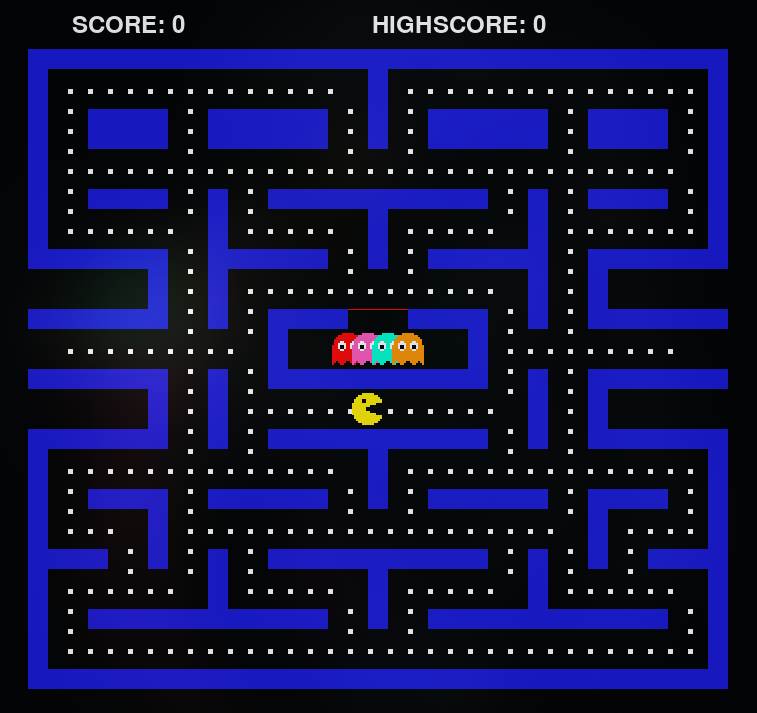
\includegraphics[width=0.82\linewidth]{assets/maze.png} % Usa una tua immagine di Pac-Man
			
			\vspace{-1em}

			\caption{\centering \small Pac-Man environment}
		\end{figure}

		\vspace{-1em}
	\end{minipage}

	Instead of traditional programming, we use an evolutionary approach to \textbf{discover} these strategies automatically.
\end{frame}

% --- Slide 2: Our Tool: NEAT ---
\begin{frame}{Our Tool: NeuroEvolution of Augmenting Topologies}
		We use \textbf{NEAT} \cite{stanley2002evolving}, a powerful algorithm that evolves both the \textbf{weights} and the \textbf{structure (topology)} of neural networks.

		Key features of NEAT:
		\begin{itemize}
			\item \textbf{Complexification:} Starts with simple networks and gradually adds nodes and connections.
			\item \textbf{Innovation Numbers:} Tracks the historical origin of genes to solve the "competing conventions problem" during crossover.
			\item \textbf{Speciation:} Groups similar networks to protect new innovations until they're ready to compete.
		\end{itemize}

		\vspace{-1em}
		
		\begin{figure}
			\centering
			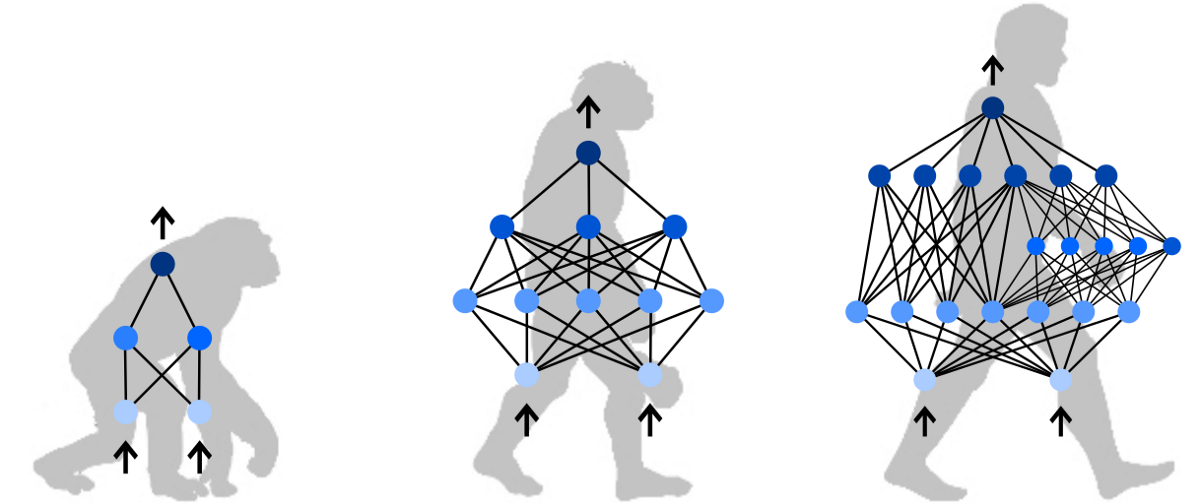
\includegraphics[width=0.5\linewidth]{assets/neat-evolution.png}
			\vspace{-1em}
			\caption{NEAT increases network complexity over time \cite{shrestha2025reinforced}.}
		\end{figure}

\end{frame}

% --- Slide 3: Project Architecture ---
\begin{frame}{Project Architecture}
	The project integrates the NEAT algorithm with a custom Pac-Man game environment.
	
	\vspace{0.5em}

	\begin{columns}[T]
		\begin{column}{0.5\textwidth}
			\textbf{Pac-Man Game Engine}
			\begin{itemize}
				\item Adapted from the \textit{PyPacman} repository.
				\item Refactored game state management for stability and performance in a machine learning context.
				\item Core logic encapsulated in a Gym-like environment.
			\end{itemize}
		\end{column}
		\begin{column}{0.5\textwidth}
			\textbf{NEAT Framework}
			\begin{itemize}
				\item \texttt{trainer.py}: Manages the evolutionary loop, population, and checkpoints.
				\item \textbf{Parallel Evaluation:} Uses Python's multiprocessing to evaluate hundreds of genomes simultaneously, drastically reducing training time.
			\end{itemize}
		\end{column}
	\end{columns}
	
	\begin{figure}
	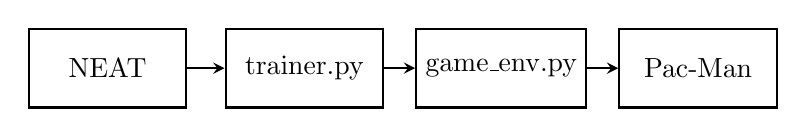
\begin{tikzpicture}[node distance=2.5cm, >=stealth, thick]
		\node (neat) [draw, rectangle, minimum width=2cm, minimum height=1cm] {NEAT};
		\node (trainer) [draw, rectangle, minimum width=2cm, minimum height=1cm, right of=neat] {trainer.py};
		\node (game_env) [draw, rectangle, minimum width=2cm, minimum height=1cm, right of=trainer] {game\_env.py};
		\node (pacman) [draw, rectangle, minimum width=2cm, minimum height=1cm, right of=game_env] {Pac-Man};
		\draw[->] (neat) -- (trainer);
		\draw[->] (trainer) -- (game_env);
		\draw[->] (game_env) -- (pacman);
	\end{tikzpicture}
	\caption{High-level interaction between NEAT and the game environment.}
	\end{figure}
\end{frame}

\begin{frame}{Choosing a Game Environment}
	
	To train and evaluate NEAT agents, a reliable Pac-Man environment was essential. After surveying available options, I selected the \textit{PyPacman} repository~\cite{pypacman} for its simplicity and open-source nature.

	\vspace{0.5em}
	\begin{columns}[T]
		\begin{column}{0.48\textwidth}
			\textbf{Advantages:}
			\begin{itemize}
				\item Lightweight and easy to understand
				\item Fully open-source and modifiable
				\item Minimal dependencies
			\end{itemize}
			\textbf{Why this matters:}
			\begin{itemize}
				\item Fast simulation of thousands of games per generation
				\item Easy integration with custom agent logic
			\end{itemize}
		\end{column}
		\begin{column}{0.48\textwidth}
			\textbf{Limitations:}
			\begin{itemize}
				\item Contained several bugs and inconsistencies
				\item Not optimized for large-scale, automated runs
			\end{itemize}
			\textbf{Actions Taken:}
			\begin{itemize}
				\item Refactored core game logic for stability and speed
				\item Added a Gym-like interface for agent-environment interaction
			\end{itemize}
		\end{column}
	\end{columns}

	The repository provided a solid foundation, but required several changes to meet the needs of this project.

\end{frame}
\section{Problem Formulation}

% --- Slide 1: How Does Pac-Man "See"? ---
\begin{frame}{How Does Pac-Man "See"? The Observation Model}
	For the neural network to make a decision, it needs a numerical representation of the game state. This is the \textbf{observation vector}.
	\vspace{1em}
	
	\textbf{Vectorial Observation Vector (26 inputs):}
	
	\begin{table}[h!]
	\centering
	\begin{tabular}{|l|l|c|}
	\hline
	\textbf{Feature} & \textbf{Description} & \textbf{\# items} \\
	\hline
	Ghost Relative Positions & $(x, y)$ for each ghost          & 8 \\
	Ghost Scared Status      & 1 bit per ghost                  & 4 \\
	Closest Dot Vector       & $(x, y)$ to nearest dot          & 2 \\
	Closest Power-up Vector  & $(x, y)$ to nearest power-up     & 2 \\
	Remaining Dots           & Number of dots left              & 1 \\
	Wall Distances           & Distance in 4 directions         & 4 \\
	Power-up Active          & 1 if power-up is active          & 1 \\
	Last Action              & One-hot, previous move           & 4 \\
	\hline
	\end{tabular}
	\caption{Total: 26 elements. \textit{Limitation: lacks spatial context.}}
	\end{table}
\end{frame}

\begin{frame}{Minimap Observation Vector (64 inputs):}
	
    The observation shown above was soon found to be ineffective. To give more awareness of the environment, I implemented an 8x8 minimap centered on Pac-Man.

    \vspace{-0.5em}

    \begin{minipage}{0.4\textwidth}
        \centering
        \vspace{0.5em}
        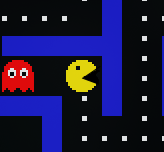
\includegraphics[width=0.8\linewidth]{assets/minimap.png}
    \end{minipage}
    \hspace{0.5em}
    \begin{minipage}{0.5\textwidth}
        \scriptsize
        $$
        \begin{bmatrix}
        \green{0.5} & \green{0.5} & \green{0.5} & 0 & 0 & \blue{-1} & \green{0.5} & 0 \\[0.5em]
        0 & 0 & 0 & 0 & 0 & \blue{-1} & \green{0.5} & 0 \\[0.5em]
        \blue{-1} & \blue{-1} & \blue{-1} & \blue{-1} & \blue{-1} & \blue{-1} & \green{0.5} & 0 \\[0.5em]
        0 & 0 & 0 & \yellow{0} & \yellow{0} & \blue{-1} & \green{0.5} & 0 \\[0.5em]
        \red{-0.75} & 0 & 0 & \yellow{0} & \yellow{0} & \blue{-1} & \green{0.5} & 0 \\[0.5em]
        \blue{-1} & \blue{-1} & \blue{-1} & \green{0.5} & 0 & \blue{-1} & \green{0.5} & 0 \\[0.5em]
        0 & 0 & \blue{-1} & \green{0.5} & \green{0.5} & \green{0.5} & \green{0.5} & \green{0.5} \\[0.5em]
        0 & 0 & \blue{-1} & \green{0.5} & 0 & 0 & \green{0.5} & 0 \\[0.5em]
        \end{bmatrix}
        $$
    \end{minipage}


    It encodes the positions of walls (\small\blue{-1}\normalsize), dots (\small\green{0.5}\normalsize), and ghosts (\small\red{-0.75}\normalsize). The four central cells represent the current Pac-Man position.

    \vspace{0.5em}

    The final observation vector is the concatenation of the vectorial observation and the minimap observation, for a total of \textbf{90 elements}.
\end{frame}

% --- Slide 2: How Does Pac-Man "Learn"? ---
\begin{frame}{How Does Pac-Man "Learn"? The Reward Function}
	The agent's goal is to maximize its cumulative \textbf{reward}. The design of the reward function—\textit{reward shaping}—is critical to guide its behavior.
	\vspace{1em}
	
	\textbf{A naive approach is insufficient:}
	\begin{itemize}
		\item \textit{Reward only for points?} The agent might learn to get stuck in a safe corner, doing nothing.
		\item \textit{Reward only for survival?} The agent might learn to run in circles and never eat dots.
	\end{itemize}
	
	\vspace{1em}
	\textbf{The Challenge:} How do we design a task that is simple enough to be learned, yet complex enough to lead to intelligent behavior?
	
\end{frame}

\begin{frame}{Early Issues: Unintended Behaviors}
	Initial experiments with complex environments and reward functions led to classic AI failures:
	
	\begin{columns}[T]
		\begin{column}{0.48\textwidth}
			\textbf{Reward Hacking}
			
            The agent found loopholes in the reward function. For instance:
                \begin{itemize}
                    \item If the reward function penalizes being stuck, the agent learns to oscillate between two positions.
                    \item If there is no cost of life, the agent learns to run in circles.
                \end{itemize}

		\end{column}
		\begin{column}{0.48\textwidth}
			\textbf{Premature Complexity}
			\begin{itemize}
				\item Starting with the full game was overwhelming.
				\item The agent couldn't learn basic evasion while also needing to manage power-ups and complex ghost behaviors.
				\item This led to a very slow or stalled learning process.
			\end{itemize}
		\end{column}
	\end{columns}
	
	\vspace{1em}
		These challenges motivated a structured approach: 
        \begin{center}
            \textbf{Curriculum Learning}
        \end{center}
\end{frame}
\section{Curriculum Learning}

% --- Slide 1: The Concept ---
\begin{frame}{The Concept of Curriculum Learning}
	\textbf{Curriculum Learning} is a training strategy where the agent is exposed to tasks of increasing difficulty, much like a human student.
		
		\vspace{0.5em}
		Rather than facing the full complexity of the final task immediately, we decompose it into a progression of easier, more manageable sub-tasks.
		
		\begin{center}
		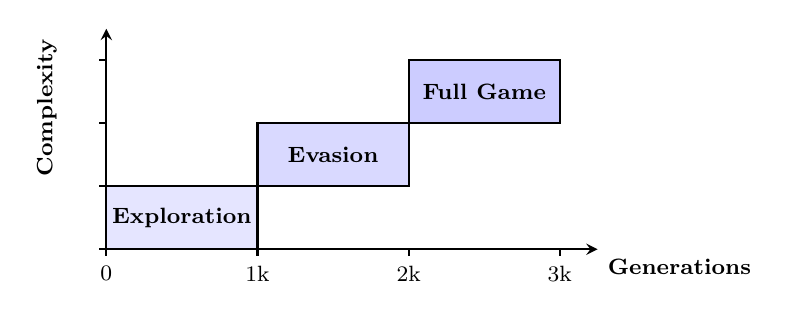
\begin{tikzpicture}[scale = 0.8, x=1.2cm, y=1cm, >=stealth, thick]
			% Draw axes
			\draw[->] (0,0) -- (6.5,0) node[below right] {\footnotesize \textbf{Generations}};
			\draw[->] (0,0) -- (0,3.5) node[above left, rotate=90, yshift=0.5cm] {\footnotesize \textbf{Complexity}};
			
			% Draw steps
			\draw[fill=blue!10] (0,0) rectangle (2,1);
			\draw[fill=blue!15] (2,1) rectangle (4,2);
			\draw[fill=blue!20] (4,2) rectangle (6,3);

			% Step labels
			\node[align=center] at (1,0.5) {\footnotesize \textbf{Exploration}};
			\node[align=center] at (3,1.5) {\footnotesize \textbf{Evasion}};
			\node[align=center] at (5,2.5) {\footnotesize \textbf{Full Game}};

			% Axis ticks and labels (optional, for clarity)
			\foreach \x/\label in {0/0, 2/1, 4/2, 6/3}
				\draw (\x,0) -- (\x,-0.1) node[below] {\footnotesize \ifnum\x=0 0 \else \ifnum\x=2 1k \else \ifnum\x=4 2k \else \ifnum\x=6 3k \fi\fi\fi\fi};

			\foreach \y/\label in {0/0, 1/1, 2/2, 3/3}
				\draw (0,\y) -- (-0.1,\y);

		\end{tikzpicture}
		\end{center}

		\vspace{0.5em}

		The hypothesis is that by mastering fundamental skills first (like exploration), the agent can build upon that knowledge to solve more complex problems (like evasion, power-up usage, etc.).
	
\end{frame}

\begin{frame}{Our Pac-Man Curriculum}
	The training was divided into automated phases, controlled by the generation number.

	\begin{itemize}
		\pause
		\setlength\itemindent{-1em}
		\item<1-> \textbf{Phase 1: Exploration Training (Gen 0-999)}
		\begin{itemize}
			\setlength\itemindent{-1em}
			\item \textbf{Goal:} Master map exploration.
			\item \textbf{Setup:} No power-ups, no ghosts, only dots.
			\item \textbf{Reward:} Simple function rewarding dot collection and penalizing time.
			\item \textbf{Key Tweak (Gen 500):} Switched from Feed-Forward to \textbf{Recurrent Networks} to enable memory.
		\end{itemize}
		\pause

		\vspace{0.5em}

		\item<2-> \textbf{Phase 2: Evasion Training (Gen 1000-1999)}
		\begin{itemize}
			\setlength\itemindent{-1em}
			\item \textbf{Goal:} Ghosts are introduced.
			\item \textbf{Setup:} Only dots and ghosts. Still no power-ups.
			\item \textbf{Reward:} The same simple reward function.
			\item \textbf{Key Tweak (Gen 1500):} Introduced scatter mode for ghosts.
		\end{itemize}
		\pause

		\vspace{0.5em}

		\item<3-> \textbf{Phase 3: Full Game Mastery (Gen 2000+)}
		\begin{itemize}
			\setlength\itemindent{-1em}
			\item \textbf{Goal:} Master the complete game.
			\item \textbf{Setup:} The full game, including power-ups.
			\item \textbf{Reward:} A highly-shaped, complex reward function is activated.
		\end{itemize}
	\end{itemize}
\end{frame}

\begin{frame}{The Advanced Reward Function (Phase 3)}
	To encourage mastery, the final reward function included several components:
	
	\begin{itemize}
		\item \textbf{Dynamic Point Multiplier:} \texttt{SCORE\_MULTIPLIER} increases as more dots are eaten, incentivizing level completion.
		\item \textbf{Event Bonuses:} Large, distinct rewards for eating dots, power-ups, and scared ghosts.
		\item \textbf{Ghost Proximity Shaping:}
		\begin{itemize}
			\item Small \textbf{penalty} for being near a dangerous ghost.
			\item Small \textbf{reward} for chasing a scared ghost.
		\end{itemize}
		\item \textbf{Exploration Bonus:}
		\begin{itemize}
			\item A small \textbf{reward} for visiting a new tile for the first time.
			\item A large \textbf{penalty} for revisiting the same tile.
		\end{itemize}
		\item \textbf{Penalties:}
		\begin{itemize}
			\item Getting stuck against a wall.
			\item Taking too long to eat the next dot (anti-stalling).
			\item A large penalty for dying.
		\end{itemize}
	\end{itemize}
\end{frame}
\section{Results}

\begin{frame}{Fitness Evolution Across the Curriculum}
	The fitness graph clearly shows the impact of our curriculum learning.
	
	\begin{figure}
		\centering
		\includegraphics[width=\linewidth]{assets/fitness.png}
		\vspace{-2em}
		
		\caption{Best fitness per generation. Vertical lines mark curriculum phases.}
	\end{figure}
\end{frame}

\begin{frame}{Analysis of Emergent Behaviors}
	Analysis of the top-performing agents across curriculum phases reveals a progression in strategy:

	\textbf{Early Generations (Exploration)}
	\begin{itemize}
		\setlength\itemindent{-1em}
		\item Agents acquire basic \bfit{navigation skills}.
		\item Tend to become \bfit{stuck against walls} or exhibit \bfit{oscillatory behavior}.
	\end{itemize}

	\textbf{Mid Generations (Evasion)}
	\begin{itemize}
		\setlength\itemindent{-1em}
		\item Agents begin to \bfit{evade ghosts}, despite little improvement in fitness.
		\item The transition to scatter mode represents the most challenging phase due to \bfit{stochasticity}.
	\end{itemize}
	
	\textbf{Late Generations (Full Game)}
	\begin{itemize}
		\setlength\itemindent{-1em}
		\item Agents gradually adapt to the revised reward structure.
		\item Demonstrate \bfit{improved ghost avoidance} compared to earlier phases.
		\item Continue to \bfit{struggle with effective use of power-ups}.
	\end{itemize}
\end{frame}

\begin{frame}{The Best Genome in Action}

	A demonstration of the final agent's performance, showcasing its ability to navigate, evade, and clear the majority of the level.

	\begin{center}
		\begin{tikzpicture}
			\node[inner sep=0pt] (img) {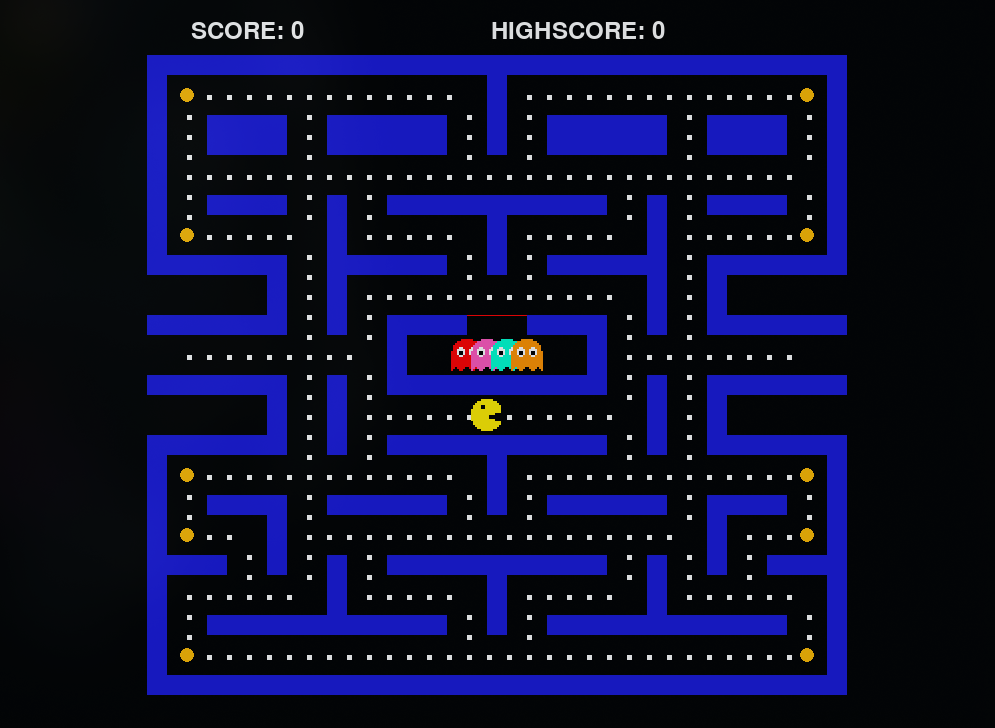
\includegraphics[width=0.7\linewidth]{assets/thumbnail.png}};
			\node at (img.center) {
				\href{https://streamable.com/klb2iw}{
					\begin{tikzpicture}
						% Make the triangle longer and larger
						\filldraw[fill=gray, opacity=0.7, draw=none] (0.7,0) -- (-0.5,0.5) -- (-0.5,-0.5) -- cycle;
					\end{tikzpicture}
				}
			};
		\end{tikzpicture}
	\end{center}
	
\end{frame}


\begin{frame}{Performance Plateau and Model Limitations}
Agents achieve high scores but never ends the level, often getting stuck in "safe" corners, especially the top-left, rather than exploring the maze. Power-ups further reinforce this risk-averse behavior.

Key limitations:

	\begin{itemize}
		\item \bfit{Perception bottleneck:} The 8x8 minimap restricts the agent's view, limiting planning and awareness.
		\item \bfit{No global planning:} The agent cannot avoid traps or optimize routes without a broader perspective.
		\item \bfit{Reward shaping:} The reward function may favor safe, suboptimal strategies like corner camping.
		\item \bfit{Potential improvements:} Richer observations and refined rewards could promote more effective behaviors.
	\end{itemize}
\end{frame}
\section{Conclusions}

\begin{frame}{Conclusions}
	\begin{itemize}
		\item \textbf{NEAT is highly effective:} 
		
		The NEAT algorithm allowed us to evolve neural networks that performed well at playing Pac-Man.
		\vspace{1em}
		\item \textbf{Gradual training leads to better results:}
		
		Training the agent in stages encouraged it to learn more advanced behaviors, such as avoiding ghosts and collecting pellets efficiently. These skills did not emerge when trying to train everything at once.
		\vspace{1em}
		\item \textbf{The agent's view limits its performance:} 
		
		Since the agent could only see a small part of the maze at a time, it often made the same mistakes in certain locations.
	\end{itemize}
\end{frame}

\begin{frame}{Future Work}
	To achieve a perfect score and consistently clear the level, several enhancements could be explored:
	
	\begin{enumerate}
		\setlength\itemindent{-0.5em}
		\item \textbf{Enhanced Observation Space:}
		\begin{itemize}
			\setlength\itemindent{-1.5em}
			\item Increase the minimap size (e.g. 16x16) for a wider field of view.
			\item Provide the agent the entire game grid (increase complexity).
		\end{itemize}

		\vspace{0.5em}

		\item \textbf{Headless, Pygame-Independent Environment:}
		
		Rewrite the game loop in pure Python/NumPy to remove the Pygame overhead; this would drastically speed up training.
		
		\vspace{0.5em}

		\item \textbf{More Granular Curriculum:}
		
		Introduce stages where ghost speed or intelligence gradually increases over generations.

		\vspace{0.5em}

		\item \textbf{Stochasticity:}
		
		Introduce stochastic elements by randomizing the agent's starting positions. This will encourage the model to develop strategies that are effective throughout the entire maze, rather than favoring specific areas.

	\end{enumerate}
\end{frame}

% ------------------------------- Bibliography? ------------------------------ %
\begin{frame}[allowframebreaks]{References}

  \bibliography{references}
  \bibliographystyle{abbrv}
  
\end{frame}

% --------------------------------- Question --------------------------------- %
{\setbeamercolor{palette primary}{fg=white, bg=bluscuro}
\begin{frame}[standout]
  \fontsize{18pt}{16pt}\selectfont
  Thank You!
\end{frame}
}
\end{document}
